\documentclass[headings=standardclasses, abstract=true]{scrartcl}

\usepackage{graphicx} % Required for inserting images
\usepackage[sorting=none, style=science]{biblatex} % Required for bibliography
\usepackage{amsmath} % For math equations
\usepackage{minted} % For code blocks
\usepackage[framemethod=TikZ]{mdframed} % For code blocks
\usepackage[svgnames]{xcolor} % For colors
\usepackage{fontspec} % For custom fonts
\usepackage{caption} % For subfigures
\usepackage{subcaption} % For subfigures
\usepackage[
    top=3cm,
    bottom=3cm,
    left=3cm,
    right=3cm
]{geometry} % Required for setting the page size
\usepackage[
    pdfauthor={Sina Atalay, Sacha Escudier, Kentaro Hanson},
    pdftitle={FastFEM v0.0.1},
    hidelinks=true
]{hyperref} % Required for hyperlinks and metadata

% Path to the bibliography file:
\addbibresource{../docs/assets/bibliography.bib}

% For Python blocks:
\newmdenv[
    outerlinewidth=1,
    outerlinecolor=Gainsboro,
    middlelinewidth=0,
    backgroundcolor=GhostWhite,
    roundcorner=3pt,
    innerbottommargin=12pt,
    innertopmargin=12pt,
    innerleftmargin=12pt,
    innerrightmargin=12pt,
    skipbelow=-0pt
]{pythonbox}
\newfontfamily\vscodefont{Droid Sans Mono}[NFSSFamily=VSCode]
\newcommand{\pythonCodeBlock}[3]{%
    \begin{figure}
        \centering
        \begin{pythonbox}
            \inputminted[fontfamily=VSCode, fontsize=\scriptsize]{python}{#1}
        \end{pythonbox}
        \caption{#2}
        \label{#3}
    \end{figure}
}


\title{\texttt{FastFEM v0.0.1}}
\subtitle{
    A Python package for solving PDEs with the finite element method    \\
    \vspace{0.2cm}
    \href{https://fastfem.com}{fastfem.com}
}
\author{
    Sina Atalay\textsuperscript{1*}, Sacha Escudier\textsuperscript{1*}, Kentaro Hanson\textsuperscript{1*} \\
    {\footnotesize \textsuperscript{1}Princeton University, Princeton, NJ, USA}\\
    {\footnotesize \textsuperscript{*}All authors contributed equally}
}
\date{
    \normalsize December 2024
}


\begin{document}

\maketitle

\begin{abstract}
\noindent Lorem ipsum dolor sit amet, consectetur adipiscing elit. Vestibulum congue gravida sem non dictum. Aenean sit amet mi fermentum ante laoreet dictum sit amet a magna. Praesent sed aliquet dui. Vivamus scelerisque condimentum mauris id euismod. Duis elementum urna eu rutrum mattis. Donec fermentum, risus et viverra aliquet, ante sapien consequat augue, sit amet dictum est nisl id elit. Proin dapibus congue tincidunt. Pellentesque habitant morbi tristique senectus et netus et malesuada fames ac turpis egestas. Fusce felis eros, aliquam sed dui ut, tempor condimentum neque. Donec quis sapien bibendum, faucibus urna sed, gravida felis. Praesent et quam ligula. Aliquam ac est eu odio tincidunt volutpat a in augue. Maecenas fermentum velit felis, vel viverra dui scelerisque pharetra. Nullam eros lorem, finibus pulvinar eleifend eu, pulvinar ac ipsum. Sed velit neque, venenatis sit amet urna vitae, vulputate ullamcorper est.
\end{abstract}

\section{Introduction}

Partial differential equations (PDEs) are the fundamental tools for mathematically modeling natural phenomena. Many fundamental phenomena observed in nature, such as general relativity\supercite{Marolf2001}, quantum mechanics \supercite{Feit1982}, heat diffusion\supercite{Bergman2011}, fluid mechanics\supercite{Lukaszewicz2016}, pricing of financial derivative contracts\supercite{Barles1998}, structural analysis\supercite{Boresi2002}, and electromagnetism\supercite{Griffiths2017}, are described by PDEs. However, most of these PDEs do not have closed-form solutions, especially in complex geometries. Therefore, engineers have developed many numerical methods for solving PDEs. One of the most popular numerical methods among them is the finite-element method (FEM), which originated in the early 1940s\supercite{Liu2022}. FEM is capable of solving non-linear PDEs in highly complex geometries. Since the 1940s, FEM has undergone significant advancements and has revolutionized the way scientific modeling and engineering design. Today, it is widely used in many industrial applications.

Currently, there are many open-source FEM software out there\supercite{fem_getdp, fem_agros, fem_calculix, fem_elmerfem, fem_freefem, fem_goma, fem_fenicsx, fem_dealii}. With \texttt{FastFEM}\supercite{fastfem}, we attempt to develop another open-source FEM software package with the goal of

\begin{itemize}
    \item Creating an easy-to-use and clean Python interface
    \item Using modern tools like JAX\supercite{jax2018github} for advanced array computing with automatic differentiation capabilities
\end{itemize}

One of the motivations for creating a Python interface was the capability of the language to create very intuitive-to-use interfaces. A modern Python interface can offer users a great way of describing FEM problems. The other motivation was leveraging the existing scientific Python environment. Python's popularity in the scientific world is still increasing, and modern libraries with state-of-the-art technologies like JAX, PyVista\supercite{Sullivan2019}, etc., are being developed.


FastFEM is planned to be a big project, but as the goal of \texttt{v0.0.1}, we decided to focus on 2D parabolic PDEs. Parabolic PDEs, such as the heat diffusion equation, Poisson's equation, and the Black-Scholes equation, are very common in various applications. A 2-dimensional parabolic PDE can be expressed as

\begin{equation}
    \frac{\partial^2 f(x,y,t)}{\partial x^2} + \frac{\partial^2 f(x,y,t)}{\partial y^2}
    =
    h(f) \frac{\partial f(x,y,t)}{\partial t} + g(x,y)
    \label{pde}
\end{equation}
where $f(x,y,t)$, $h(f)$, and $g(x,y)$ are scalar functions, $x$ and $y$ are spatial coordinates, and $t$ is time.

Currently, \texttt{FastFEM v0.0.1} can
\begin{enumerate}
    \item create a 2D mesh,
    \item take initial conditions, boundary conditions, h(f), and g(x,y) as inputs,
    \item solve \autoref{pde} with FEM, and
    \item plot the solution.
\end{enumerate}


In this report, the theory behind FEM is summarized. The features and capabilities of \texttt{FastFEM v0.0.1} are presented. Some example results are shown. Finally, the conclusion and outlook are discussed.

\section{Theory}

\section{Features and Capabilities}

This section summarizes \texttt{FastFEM v0.0.1}'s features and capabilities: mesh generation, solving parabolic PDEs with FEM using elements and fields, and plotting.

\subsection{Mesher}

\texttt{FastFEM} uses Gmsh\supercite{Gmsh} for mesh generation. Currently, \texttt{v0.0.1} offers two fundamental 2D mesh generation functions, as shown in \autoref{fig:mesh-example1}.  The results of the functions are shown in \autoref{fig:mesh}. \texttt{FastFEM} is fully statically typed so that users can get autocomplete suggestions when writing the function's arguments and using the mesh object it returns.

\pythonCodeBlock{figures/mesher-example1.py}{Two available functions of \texttt{FastFEM v0.0.1} for generating 2D square and rectangle meshes that are shown in \autoref{fig:mesh}.}{fig:mesh-example1}

\begin{figure}
    \centering
    \hfill
    \begin{subfigure}[c]{0.4\textwidth}
        \centering
        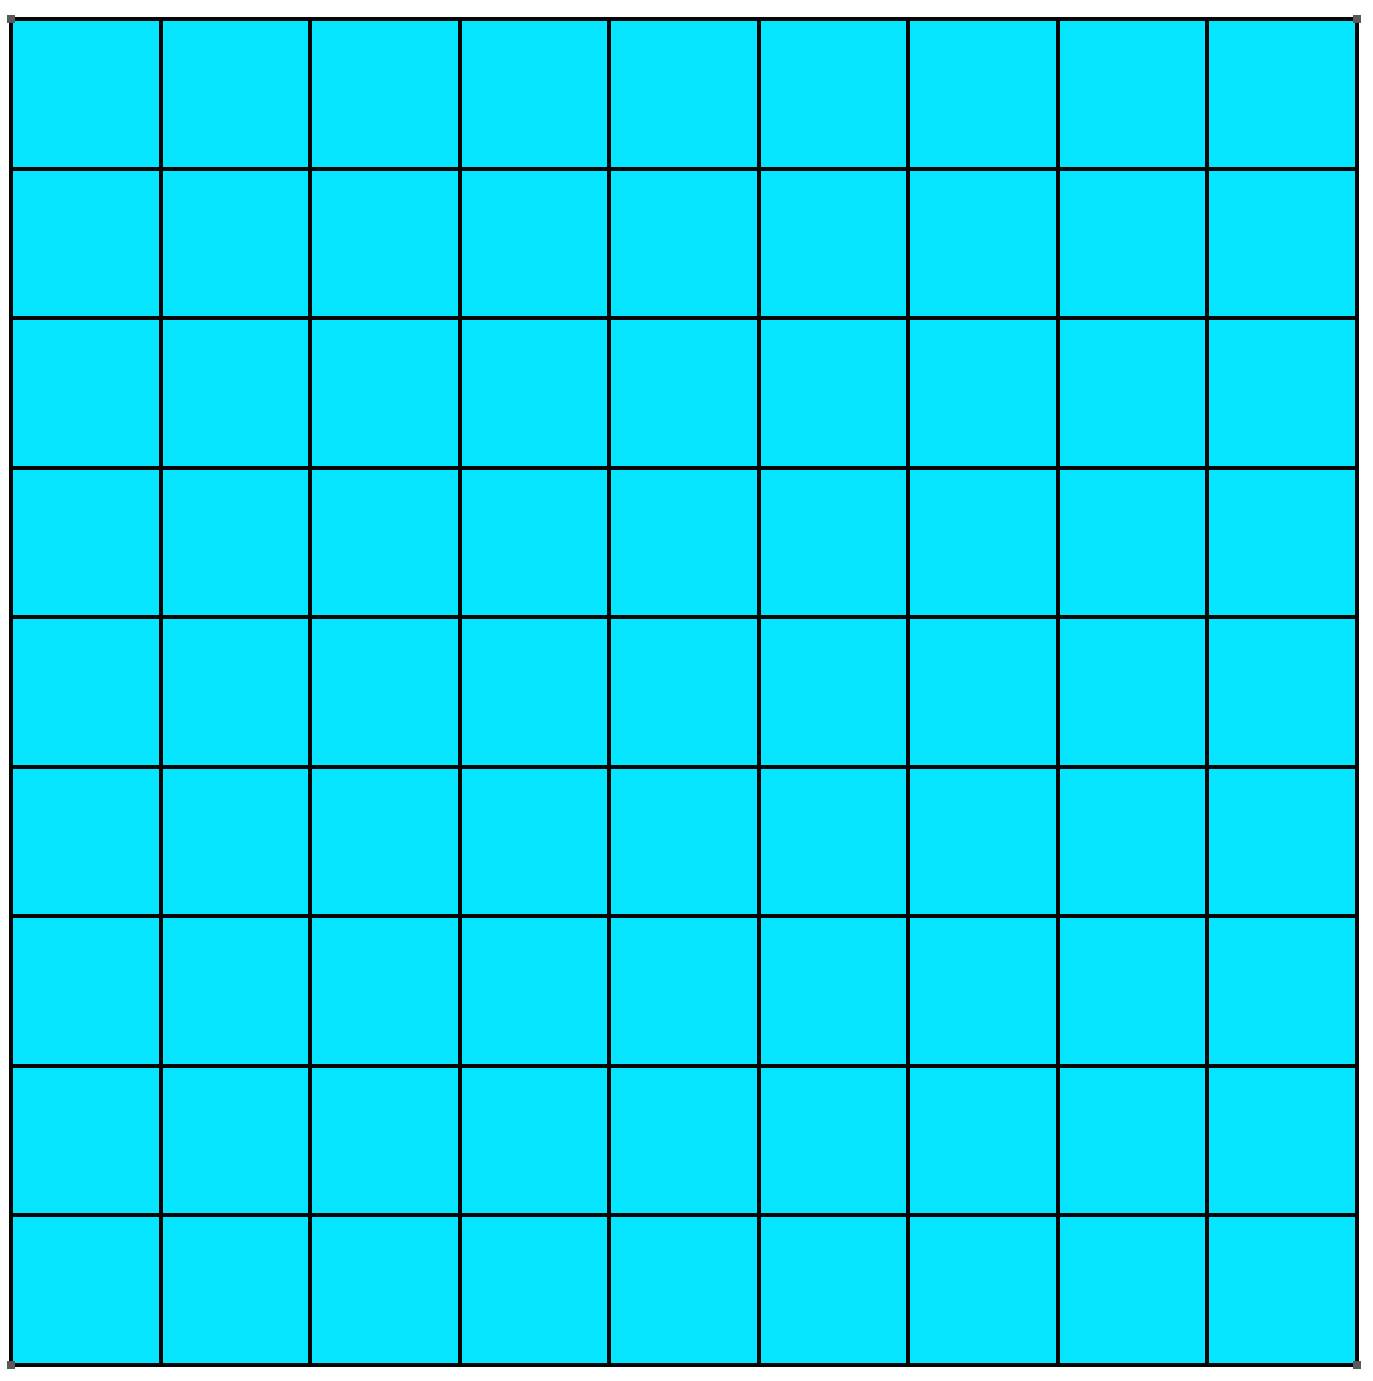
\includegraphics[width=\textwidth]{figures/square_mesh.png}

        \caption{Square mesh.}
        \label{fig:square}
    \end{subfigure}
    \hspace{0.1\textwidth}
    \begin{subfigure}[c]{0.4\textwidth}
        \centering
        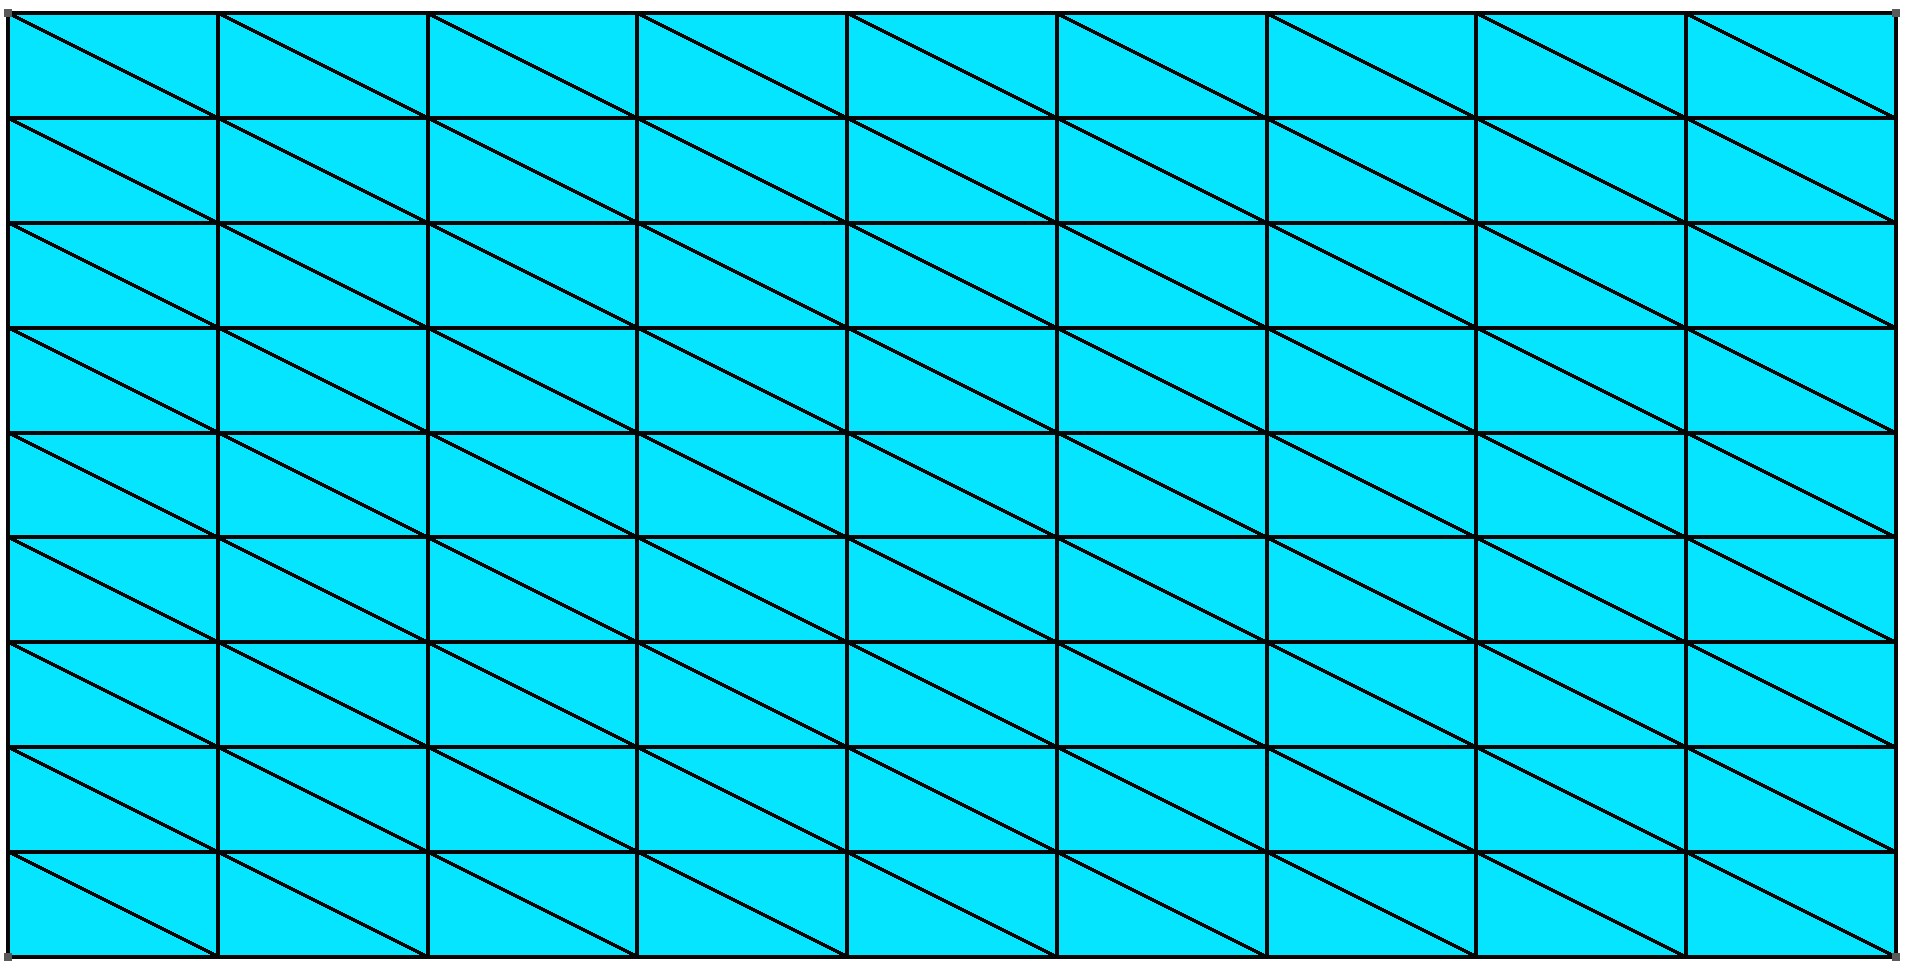
\includegraphics[width=\textwidth]{figures/rectangle_mesh.png}
        \caption{Rectangle mesh.}
        \label{fig:rectangle}
    \end{subfigure}
    \caption{Two examples of mesh generated with the functions in \autoref{fig:mesh-example1}.}
    \label{fig:mesh}
    \hfill
\end{figure}

\texttt{FastFEM v0.0.1} also provides a general-purpose, object-oriented interface for 2D mesh generation by abstracting Gmsh's functional approach. For example, a mesh of an arbitrary 2D geometry, as shown in \autoref{fig:arbitrarymesh}, can be created using the code presented in \autoref{fig:mesh-example2}.

\pythonCodeBlock{figures/mesher-example2.py}{The code that generates the mesh of an arbitrary geometry shown in \autoref{fig:arbitrarymesh}.}{fig:mesh-example2}

\begin{figure}
    \centering
    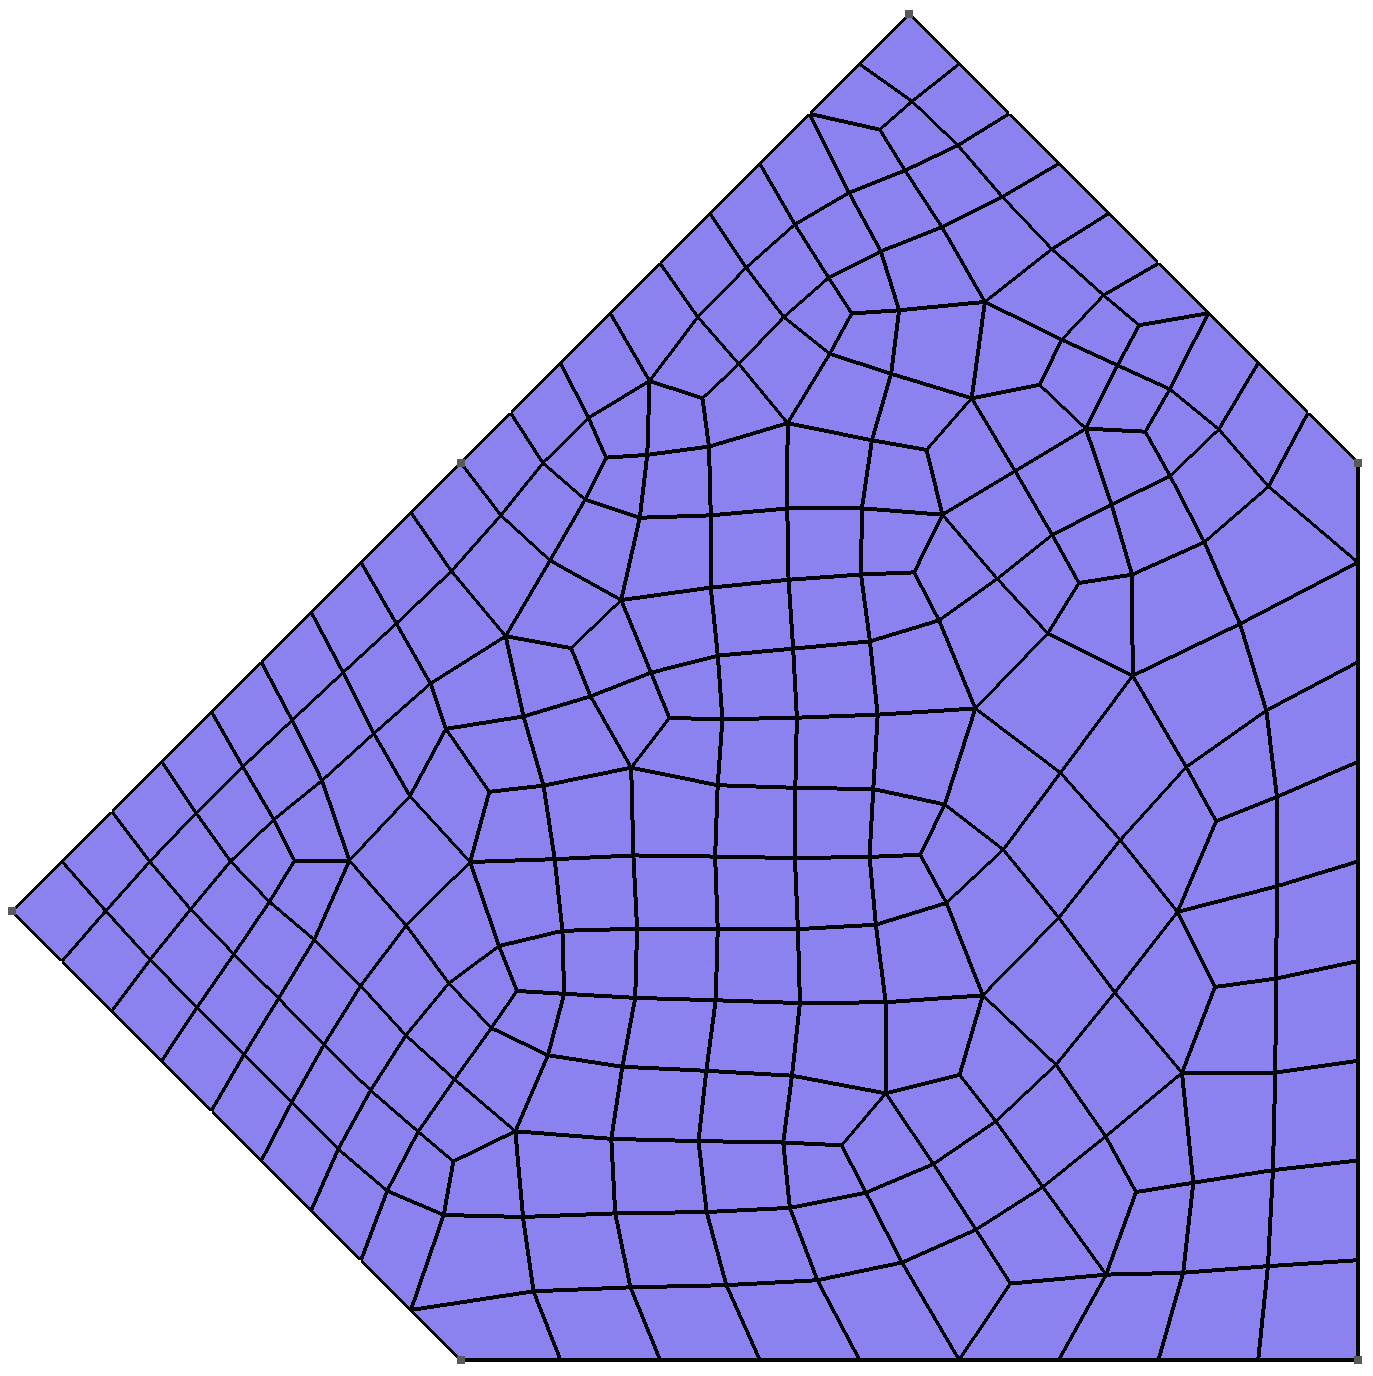
\includegraphics[width=0.5\textwidth]{figures/arbitrary_mesh.png}
    \caption{An arbitrary 2D mesh generated using the code in \autoref{fig:mesh-example2}.}
    \label{fig:arbitrarymesh}
\end{figure}

\subsection{Elements and Fields}

\subsection{Plotter}

\section{Results}

\section{Software Quality and Maintenance}

\texttt{FastFEM} is open-source and version-controlled on GitHub\supercite{fastfem}. We are following some rules to ensure high software quality for better maintainability:

\begin{itemize}
    \item Direct pushes to the "main" branch are not allowed. All the contributions should be made as a pull request.
    \item Each pull request should be reviewed by two developers, and all the automated tests should be passed before it is merged.
    \item All the documentation and reports related to the software are maintained in the same repository.
    \item All the important discussions are conducted on the issues page.
    \item The changelog is kept.
    \item Semantic Versioning 2.0.0\supercite{semanticVersioning} convention is followed for versioning.
\end{itemize}

\texttt{FastFEM} also uses many other open-source tools for various reasons:
\begin{itemize}
    \item Hatch\supercite{hatch} is used as a project manager.
    \item MkDocs\supercite{mkdocs} with Material theme\supercite{mkdocsmaterial} is used for the documentation.
    \item MkDocstrings\supercite{mkdocstrings} is used to generate API references.
    \item pytest\supercite{pytest} is used to write automated tests.
    \item GitHub Actions\supercite{githubactions} is used to run the automated tests after each update.
    \item pre-commit\supercite{precommit}, Ruff\supercite{ruff}, and Black\supercite{black} are used for linting and formatting.
    \item pre-commit.ci is used to run the linters and formatters after each update.
\end{itemize}


\section{Conclusion and Outlook}

\clearpage
\printbibliography

\end{document}